\documentclass{article}
\usepackage{amsmath}
\newcommand{\argmin}{\arg\!\min} 
\newcommand{\argmax}{\arg\!\max} 
\usepackage{amssymb}
\usepackage{amsfonts}
\usepackage[T1]{fontenc}
\usepackage{bm}
\usepackage{array}
\usepackage{graphicx}
\usepackage[utf8]{inputenc}
\usepackage{minted}

\title{Tianshou RL library - documentation notes}
\date{\today}
\author{Marko Guberina 19970821-1256}

\begin{document}
\maketitle
\section{Purpose}
Great library, has Rainbow which is what i want to use so that I don't have to code it up myself.
Also quite neat is the fact that a lot of pedestrian code like logging is already taken care of.
The problem is that it's quite involved in the sense that there are many abstractions and layers
in the library structure.
In other words, there's a lot of code to read to be able to use this thing.
As I recently found out, I can't just read complicated technical information and
remember it in a retrievable way --- hence these notes.
Hopefully they'll also be useful as a cheatsheet.

\section{Introduction via a Q-learning example}
\begin{figure}[htpb]
		\centering
		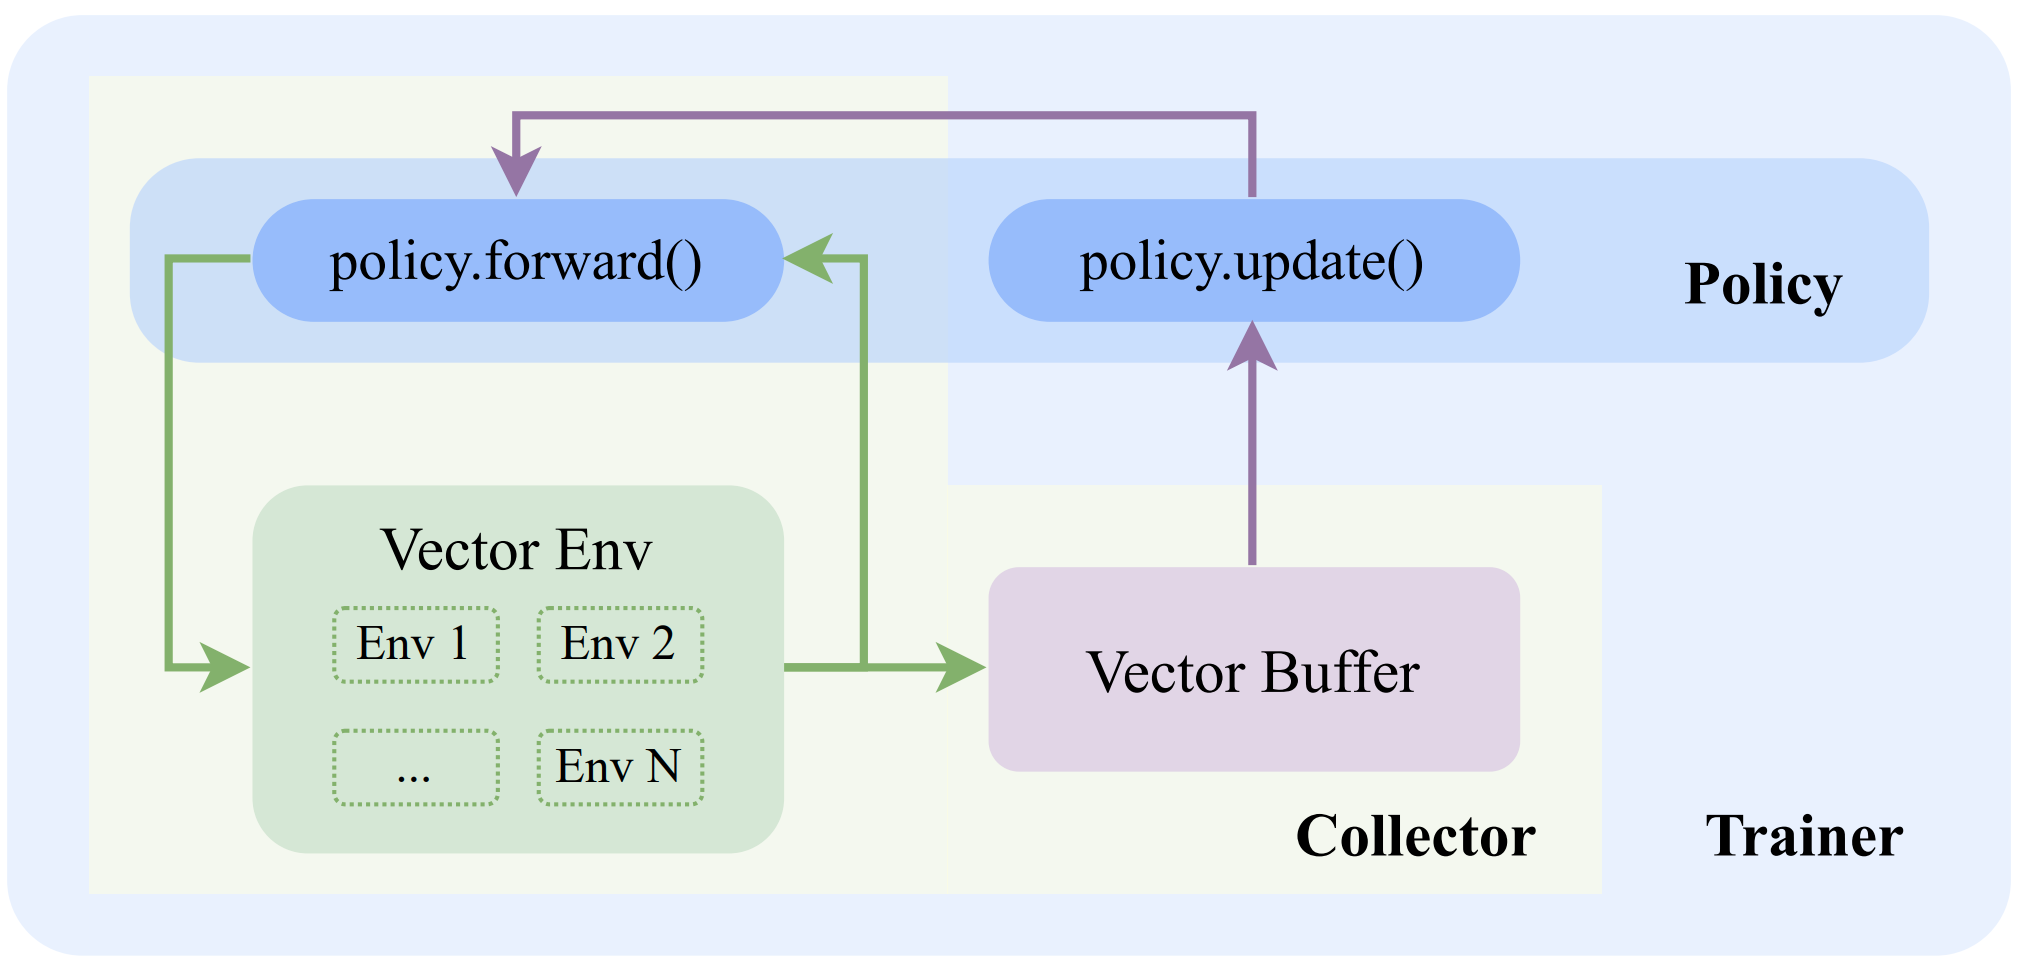
\includegraphics[width=0.8\textwidth]{"./basic_q_learning_pipeline.png"}
		\caption{basic q learning pipeline}
\end{figure}

The gym part is standard.
Tianshou supports vectorization for all environments. There are 4 types
of vectorizing environment wrappers:
\begin{enumerate}
		\item \fbox{\texttt{DummyVectorEnv}} - sequential version, using a single thread for loop
		\item \fbox{\texttt{SubprocVectorEnv}} - uses Python multiprocessing and pipes
		\item \fbox{\texttt{ShmemVectorEnv}} - uses shared memory instead of pipes
		\item \fbox{\texttt{RayVectorEnv}} - uses Ray. the only choice for computing in a cluster with multiple machines
\end{enumerate}

\textbf{Policies} and \textbf{networks} are decoupled --- you define a network and pass it to the policy you want.
The policies' code is mostly straighforward.
\textbf{Buffers} are non trivial, as their class implements sampling methods and other related functionality.
\textbf{Collectors} are a Tianshou specific thing that's very important and not straighforward.
The idea behind collectors is to manage how policies interact with the environment ---
esentially to collect and put data in buffers.

The gist of the collector code is the following:
\begin{minted}[mathescape, linenos]{python}
# the agent predicts the batch action from batch observation
result = self.policy(self.data, last_state)
act = to_numpy(result.act)
# update the data with new action/policy
self.data.update(act=act)
# apply action to environment
result = self.env.step(act, ready_env_ids)
obs_next, rew, done, info = result
# update the data with new state/reward/done/info
self.data.update(obs_next=obs_next, rew=rew, done=done, info=info) 
\end{minted}
Collectors also enable watching the agent's performance.
To do so, you create a collector to which you pass the render argument,
for example \fbox{\texttt{render = 1 / 35}} for 35 FPS.

There is also a \textbf{trainer}, which handles the training,
provided everything mentioned so far, including additional training-related parameters.
Trainer also supports TensorBoard for logging.
You just need to create the logger:
\begin{minted}[mathescape, linenos]{python}
from torch.utils.tensorboard import SummaryWriter
from tianshou.utils import TensorboardLogger
writer = SummaryWriter('log/dqn')
logger = TensorboardLogger(writer)
\end{minted}
and pass it to the trainer.



\section{Basic concepts in Tianshou}
The control flow of Tianshou's reinforcement learning agent is depicted in the following picture:
\begin{figure}[htpb]
		\centering
		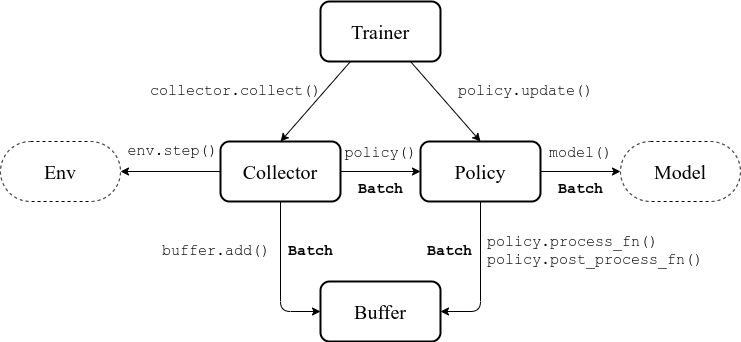
\includegraphics[width=0.8\textwidth]{"./concepts_arch2.png"}
		\caption{"concepts arch2.png"}
\end{figure}

\subsection{Batch}
\fbox{\texttt{Batch}} is designed to store and manipulate ``hierarchical named tensors''.
Hierarchical named tensors are a set of tensors whose name forms a hierarchy.
Esentially they're nested distionaries.
The reason why that's need is because states and actions vary with environments.
Consider the usual:
\begin{minted}[mathescape, linenos]{python}
state, reward, done = env.step(action)
\end{minted}
\fbox{\texttt{reward}} and 
\fbox{\texttt{done}} are mostly just scalar values.
But \fbox{\texttt{state}} can be a vector, a tensor, a camera input combined with sensory input,...
In the last case you need a hierarchical named tensor which could look like:
\begin{minted}[mathescape, linenos]{python}
{
    'done': done,
    'reward': reward,
    'state': {
        'camera': camera,
        'sensory': sensory
    }
    'action': {
        'direct': direct,
        'point_3d': point_3d,
        'force': force,
    }
}
\end{minted}

That's all fine and well, but how do you batch these things?
Enter \fbox{\texttt{Batch}}. It can be defined by using the following rules:
\begin{enumerate}
		\item a \fbox{\texttt{Batch}} can be an empty 
				\fbox{\texttt{Batch()}}, or have at leas one key-value pairs (can store keys too, but that's advanced stuff)
		\item keys are always strings corresponding to names of corresponding values
		\item values can be scalars, tensors, or \fbox{\texttt{Batch}} objects. scalars are booleans, ints, floats, the same in NumPy, None and strings
		\item both PyTorch \fbox{\texttt{torch.tensor}} and NumPy 
				\fbox{\texttt{nd.ndarray}} tensors are supported
		\item \fbox{\texttt{Batch}} can not store dicts! That's internal to 
				\fbox{\texttt{Batch}} structure.
		\item if you want something edgy, put it in an \fbox{\texttt{np.ndarray}} because they support 
				the \fbox{\texttt{np.object}} data type and that's pretty much any Python object
\end{enumerate}


There are 7 reserved keys in \fbox{\texttt{Batch}}:
\begin{enumerate}
		\item \fbox{\texttt{obs}} --- observation at step $ t  $
		\item \fbox{\texttt{act}} --- action at step $ t  $
		\item \fbox{\texttt{rew}} --- reward at step $ t  $
		\item \fbox{\texttt{done}} --- done flag at step $ t  $
		\item \fbox{\texttt{obs\_next}} --- observation at step $ t+1  $
		\item \fbox{\texttt{info}} --- info at step $ t  $
		\item \fbox{\texttt{policy}} --- data computed by policy at step $ t  $
\end{enumerate}

\subsubsection{Constructing and using \fbox{\texttt{Batch}}es}
You can construct them from \fbox{\texttt{dict}}ionaries or a list of dictionaries, but the dictionaries in
the list will automatically get stacked.
You can also do it through \fbox{\texttt{kwargs}}, i.e.
\begin{minted}[mathescape, linenos]{python}
data = Batch(a=[4, 4], b=[5, 5], c=[None, None])
\end{minted}
You can also do a combination of the two.

An element can be accessed via \fbox{\texttt{b[key]}} or \fbox{\texttt{b.key}}.
Dictionary methods, like iteration over keys also work if you need those.
Furthemore, some methods from NumPy ndarray API are available as well.
\paragraph{Note:} to be on the safe side, try out what you're doing in a shell first.
You can even stack, concatenate and split them --- the values of corresponding keys will be appended in a list of those values under
said key.

There are some advanced options which regard reserved keys and heterogenous batches, but I won't be needed those.

The most common use of \fbox{\texttt{Batch}} is to be a minibatch from a buffer storing RL experience.
Then \fbox{\texttt{Batch}} is a collection of tensors whose first dimensions are the same.
In that case, \fbox{\texttt{len(b)}} is the number of elements in the \fbox{\texttt{Batch}} \fbox{\texttt{b}}.
Likewise you can get the \fbox{\texttt{b.shape}}.
However if all leaf nodes in a \fbox{\texttt{Batch}} are tensors of different lengths, you won't get what you want!

Cool thing:
\fbox{\texttt{Batch}} is serializable and therefor pickleable.

\subsection{Buffer}
\fbox{\texttt{ReplayBuffer}} stores experience data.
It's purpose is to manage \fbox{\texttt{Batch}}.
All data is stored in a circular queue.
Let \fbox{\texttt{buf}} be a \fbox{\texttt{ReplayBuffer}}.
To add to it, do use the \fbox{\texttt{add}} member function, ex.
\fbox{\texttt{buf.add(Batch(...))}}.
You can add one buffer to another while keeping chronology with
\fbox{\texttt{buf.update(buf2)}}.
You can also use \fbox{\texttt{load}} to load it from a file.
For RNN training, you can use frame\_stack.

\subsection{Policy}
There are different classes of policies, but all policies must inherit from \fbox{\texttt{BasePolicy}}.
Typicall function are the following ones:
\begin{enumerate}
		\item \fbox{\texttt{\_\_init\_\_()}}
		\item \fbox{\texttt{forward()}} --- compute action with given observation
		\item \fbox{\texttt{process\_fn()}} --- pre-process data from the replay buffer
		\item \fbox{\texttt{learn()}} --- update policy with a given batch of data
		\item \fbox{\texttt{post\_process\_fn()}} --- pre-process data from the replay buffer
		\item \fbox{\texttt{update()}} --- this one does it all: samples from buffer,
				pre-processes data (ex. computing the n-step return),
				learn from data and post-proces sthe data (ex. update the prioritized replay buffer)
\end{enumerate}

Policies can be in the following states:
\begin{table}[htpb]
		\centering

		\begin{tabular}{l l c c }
				\textbf{Policy state} & & \textbf{\fbox{\texttt{policy.training}}} & \textbf{\fbox{\texttt{policy.updating}}} \\
				\hline
				training state & collecting state & True & False \\
				& updating state & True & True \\
				testing state & & False & False 
		\end{tabular}
\end{table}
Because sometimes you want to update the (hyper)parameters and sometimes you don't.

\fbox{\texttt{policy.forward}} is algorithm specific, but generally it is the mapping
of \fbox{\texttt{(batch, state, ...) -> batch}}.
The input batch comes from either \fbox{\texttt{collect()}} or \fbox{\texttt{sample()}}.

\subsection{Collector}
Is quite straighforward, check docs for specific names of things.

\subsection{Trainer}
Is quite straighforward, check docs for specific names of things.
Takes care of ez things like writing for loops for collector, policy updating etc..











\end{document}
